% outline background

% 1. Video games
% 2. Reinforcement learning
% 3. Deep Reinforcement Learning
% 4. Conclusion

\chapter{Background}

The following sections give an overview of the Reinforcement Learning framework
and some of its variations, provide some information about games-based
artificial intelligence environments, and finally review recent work done on
Real-Time Strategy games.

\section{Reinforcement Learning}

Reinforcement Learning is centered around the idea that a good chunk of problems
in control theory and artificial intelligence can be viewed as sequential
decision making processes. In such formalisation we consider \emph{agent} all
the parts of the problem that contribute to the execution of the decision-making
process, and \emph{environment} everything outside of the agent.  Given a
discrete-time setting, the full system is commonly framed in the following way:
at every episode $t$ the agent receives some observation $s_t \in S$ from
the environment, executes an action $a_t \in A$ derived from a policy $\pi :
S \rightarrow A$, and receives a reward $r_{t+1} \in \mathbb{R}$ together with
a new observation. The objective
of reinforcement learning algorithms usually consist in maximising the reward
received in a certain time frame using the experience gained by acting within
the environment.

\subsection{Markov Decision Processes}

The decision process becomes quickly intractable if you have to process the
entirety of the experience at every step, therefore we need a way to allow us to
approximate history without losing important information.

We define \emph{Markov Decision Process} (MDP) a task where the current
observation and reward depend entirely on the past observation-action pair
(Equation \ref{eq:rl_mdp}).

\begin{equation}
Pr(s_{t+1}, r_{t+1} | s_1, a_1, ... , s_t, a_t) = Pr(s_{t+1}, r_{t+1} |
s_t, a_t)
\label{eq:rl_mdp}
\end{equation}

The observed state $s_t$ is called the \emph{Markov State}, and is defined as
the state that summarises all gained experience up until time $t$. If during a
particular task all that the agent observes are Markov states, then the problem
is defined \emph{fully observable}, otherwise it's \emph{partially observable}.
Our work focuses on fully observable problems, but we will take partial
observability into account towards the final chapters to discuss some of the
properties of this particular subset of tasks. Additionally we assume our tasks
to be \emph{episodic}, which means that they possess a finite horizon with a
number of reachable terminal states, and that the environment and the agent have
finite action and state spaces $A$ and $S$.

In general MDPs define a transition probability $P_a(s, s')$ describing the
probability that the process might move into a new state $s'$ from state $s$
taking action $a$, and a reward function $R_a(s, s')$ that provides the expected
reward for such transition.

% reviewed till here.

\begin{equation}
P_a(s, s') = Pr(s' | s, a)
\end{equation}
\begin{equation}
R_a(s, s') = \mathbb{E}[r|s, s', a]
\end{equation}

At every step the action taken by the agent is selected by a policy $\pi(s, a) =
P_r(a | s)$, and we know that any given MDP there exist an optimal policy
$\pi^*(s, a)$ that maximises the expected total reward $R_t = \sum^T{r_t}$:

\begin{equation}
  \pi^*(s, a) = \operatornamewithlimits{argmax}_{\pi} \mathbb{E}_{\pi}[R_t | s_t]
\end{equation}

Reinforcement learning methods can also be divided in two groups with
respective to whether or not they model $P_a(s, s')$ and $R_a(s, s')$.
\emph{Model-free} reinforcement learning learn from experience without any
knowledge of environment, \emph{model-based} reinforcement learning either
assume some or full knowledge of the environment or estimate it during the
learning process.

Some of the most successful and popular reinforcement learning algorithms are
based on the idea of choosing actions depending on the \emph{value} of current
and future states. We define $V_{\pi}(s)$ and $Q_{\pi}(s, a)$ to be respectively
the expected return from state $s$ under a policy $\pi$ and the expected return
after choosing an action $a$ in $s$ before following $\pi$ (Equations
\ref{eq:value} and \ref{eq:q_act}).

\begin{equation}
V_{\pi}(s) = \mathbb{E}[R_t | s]
\label{eq:value}
\end{equation}
\begin{equation}
Q_{\pi}(s, a) = \mathbb{E}[R_t | s, a]
\label{eq:q_act}
\end{equation}

Depending on the algorithm, either or both functions are updated iteratively as
new observations arrive. Those functions can then be taken as factors into the
planning process by simple greedy policies or more complex agent systems.

% insert some examples of model-free and model-based models

All of those models unfortunately do not scale well when tackling large or
growing action spaces, as the framework itself suffers from the so-called
\emph{curse of dimensionality}. 

\subsection{Hierarchical Reinforcement Learning}

It has been shown that planning methods can
strongly benefit from including some form of hierarchical modelling, however
most classical reinforcement learning algorithms do not naturally offer a way to
incorporate hierarchies into their pipelines.

Many researchers have tried to experiment with several methods for hierarchical
reinforcement learning. Contributions have explored with changing different part
of the standard reinforcement learning process, but they have mostly focused on
adding temporal abstractions. These abstractions have for instance been used to
create forms of \emph{temporally-extended actions} such as 
\emph{behaviours},
\emph{skills}, 
\emph{options}, 
or \emph{control modes}.
Those methods involve splitting and clustering states in some way to allow
the creation of partial policies, which can then be combined using Bayesian
reasoning or some other type of control (even RL itself).

% maybe explain SMDP here

Another approach to the problem is value decomposition methods such as MAXQ,
where a hierarchy of sub-tasks in learnt and concurrently solved by decomposing
the graph until primitives are reached. The higher layers are governed by the
policy, but the available actions reduce as the algorithm walks the graph.

% Put MAXQ graph

Unfortunately all of those methods help the decision-making process by modelling
different levels of abstractions within the reinforcement learning framework,
but they don't solve the problem of engineering the state representation, making
the application of reinforcement learning algorithms to robotic and other
applied fields.

\subsection{Deep Reinforcement Learning}

Deep Reinforcement Learning aims to solve the problem of learning policies from
multi-dimensional state representations without having to manually engineer
features and the representation itself. Reinforcement learning has historically
made use of general state approximators like Artificial Neural Networks (ANNs),
but difficulties in training multi-layer architectures and the additional
learning time has stopped researchers from being able to solve the
state-engineering problem and focus purely on tackling the decision-making part.
The recent surge of Deep Learning has managed to shake the reinforcement
learning community and try to use newly developed architectures as powerful
general state approximators.

\subsubsection{Deep Learning}

Deep learning has received an increasing amount of attention in recent years.
Its usage has given rise to several powerful generative and discriminative
models that have resulted in groundbreaking performances in various applied
machine learning tasks such as speech processing, object recognition, machine
translation and more generic data analysis.

The strength of deep learning models - when compared to standard ``shallow''
approaches in machine learning - consists in the ability to concurrently learn
multiple representation of some input space, therefore allowing to effortlessly
construct models that can learn to automatically detect and extract features.
Different architectures and stacks of layers can allow to process visual input,
language sentences, raw motor data and many more dimensionally complex input
spaces.

The main issue with those new models is that they require a lot of data to
converge to a good internal representations even with modern and specialised
optimisation algorithms, however reinforcement learning generally suffers from
the same issue, which makes the two techniques relatively compatible.

We'll see in Chapter 3 that by employing some learning tricks it is in fact
possible to use deep networks to approximate a lot of the classic reinforcement
learning functions (such as for instance the value function $V_{\pi}(s)$).

\section{Videogames-based Learning Environments}

Playing video-games often involve a wide variety of transferable skills ranging
from reactive planning to reasoning under extreme uncertainty. It's probably
reasonable to state that one of the industries that has most benefited from
artificial intelligence research is in fact the computer gaming industry. AI is
regularly used to create challenging and enjoyable scenarios for human players,
and has essentially motivated a lot of the community to create algorithms and
models that can be used in a variety of contexts and that can scale efficiently
with different domains.

We will cover in particular recent platforms that allow to test a variety of
reinforcement learning algorithms and Real-Time Strategy games.

% Torcs ?

\subsection{ALE}

The Arcade Learning Environment (ALE) is a software framework developed to
easily allow the building of computer agents that can play a number of Atari
2600 games. Atari 2600 is one of the oldest video game consoles: sold from 1977
for over a decade, it was one of the first instances of computers purposely
built for gaming. Over 500 games were available at the time and the number
increases every years thanks to indie developers. ALE aims to allow developers
to use one interface to control all games, so that energy and focus can be spent
on building context-independent AI algorithms. For the moment over 60 games are
available in the platform, and most of them have been featured in reinforcement
learning and AI work. The interface is built on an open-source emulator for
Atari 2600 ROM images, and is released under the GNU GPL license.

In Chapter 3 we discuss work that managed to reach human and superhuman
performances on most of the games available in this system. In their platform
presentation paper, the authors of ALE state that once the games available in
ALE are defeated, the community should move up the ladder and challenge newer
and more complex games.

\subsection{RTS AI Research}

\begin{figure}[h]
    \centering
    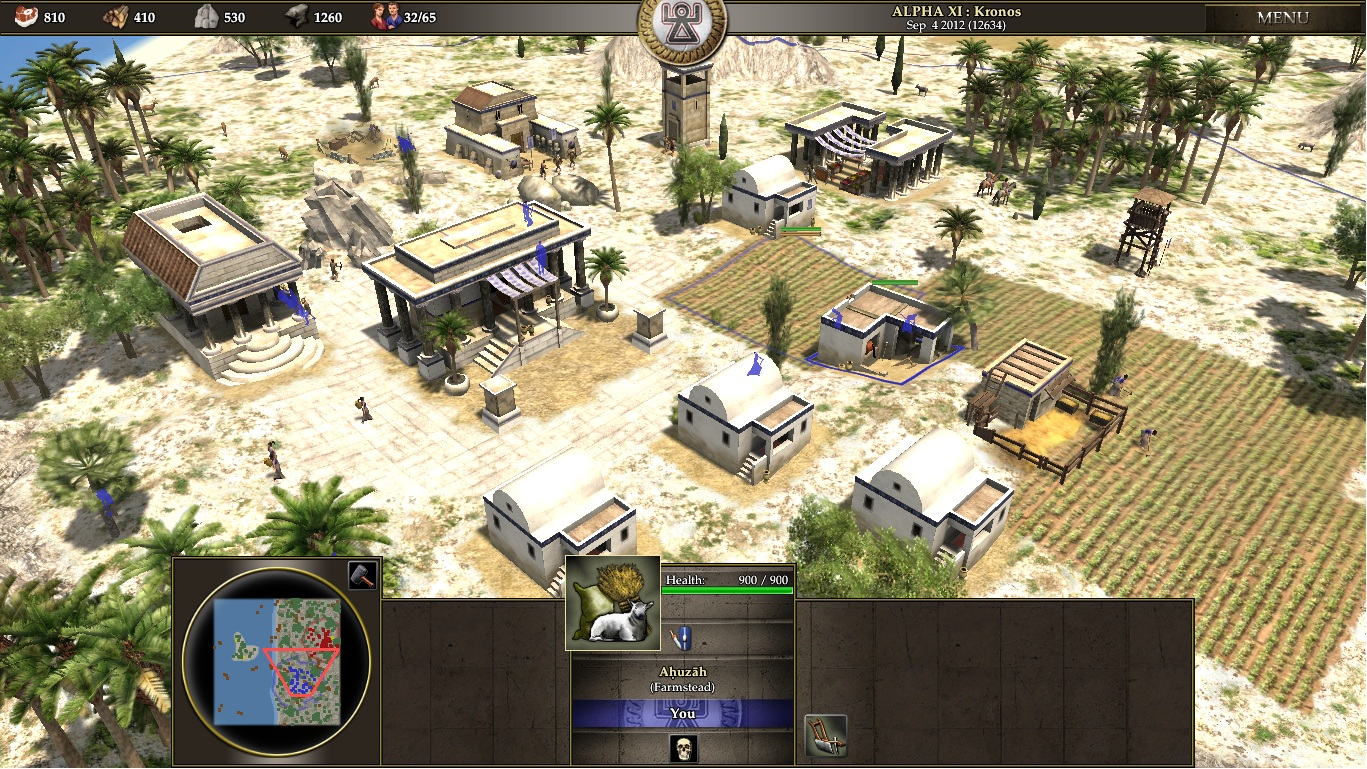
\includegraphics[width=0.9\textwidth]{ch2/0ad}
    \caption{Typical in-game view of 0 A.D., an open source cross-platform
      Real-Time Strategy game.}
    \label{fig:0ad}
\end{figure}


Real time strategy (RTS) games have historically been a source of complex
problems for AI researchers. The domain they represent is essentially a
simplified military simulation where players fight live and fight in a
fixed-size 2D map for the control of the resources lying all over the map to
build armies and an economy that allows them to win battles and finally the
overall game. The variety of AI and decision problems that this typology of
games involves and requires solving include (but are not limited to):

\begin{itemize}
  \item Decision making under uncertainty
  \item Opponent modelling and Learning
  \item Resource management
  \item Real-time planning
  \item Exploration/exploitation dilemma
\end{itemize}

Those are all terribly challenging problems that have spawned several techniques
and even entire areas of research \citep{buro2003real}. The creation of a
machine learning system that can at least partially solve all those problems and
therefore have the chance to have a fair game against a human opponent is far
from being close, even with the relatively game-changing performances of Deep
Reinforcement Learning.

In the past years several RTS research platforms have emerged, the most
prominent ones being Stratagus, OpenRTS and Wargus, however most of them lacked
the required polish and robustness to be used as AI platforms. Additionally
commercial games allow researchers to take advantage of the players community to
collect useful data, which is a critical advantage given how data-hungry most of
the current state-of-the-art machine learning systems are. A more feasible
solution is instead to take one of the popular commercial games and adapt it as
to make it an AI testing suite.

\subsection{StarCraft Brood War}

Starcraft is a relatively old commercial game developed in 1998 by Blizzard
Entertainment, Inc. that represents the quintessence of Real Time Strategy
games. Since the beginning it has attracted tens of millions of players, selling
as many copies and pioneering the use of video games as competitive e-sport
platforms. As a consequence StarCraft has been used as a platform for
professional competitions for nearly 20 years, generating annually an industry
of several millions of US dollars. When StarCraft 2 was released in 2009, the
game sold even more copies, creating another wave of excitement towards online
gaming that has yet to stop growing. With such a background it should be clear
why it's important to provide the artificial intelligence and machine learning
community a way to use the massive amount of collected playing data available
online to seriously start tackling the complexity of Real-Time Strategy games.

\begin{figure}[h]
    \centering
    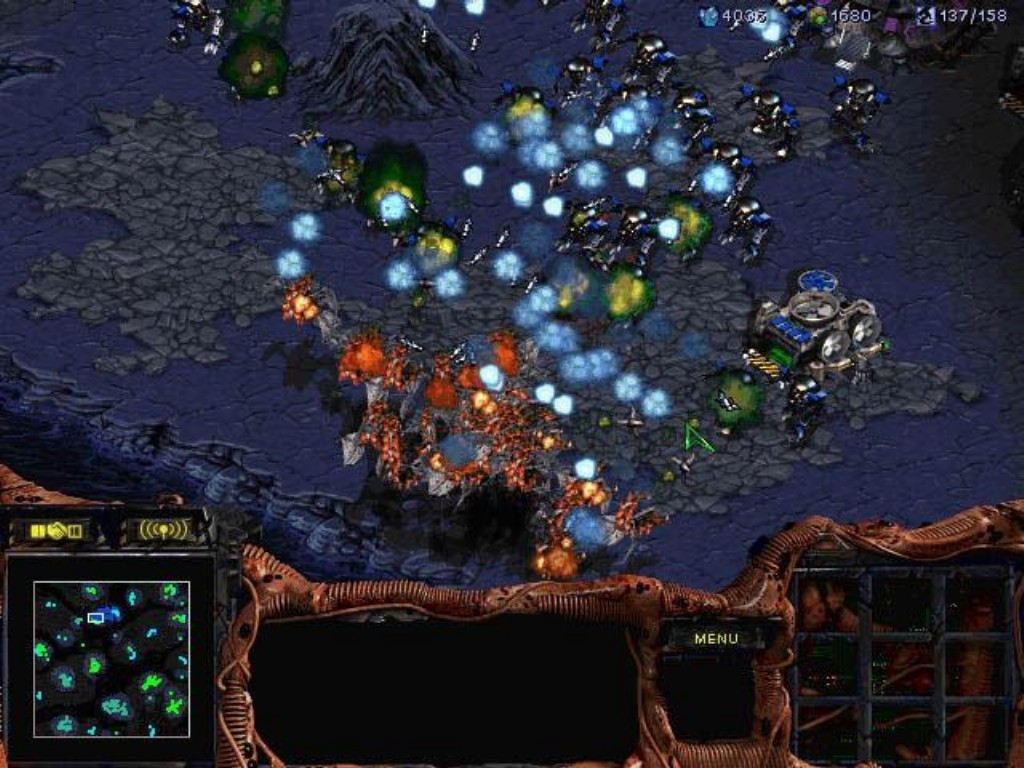
\includegraphics[width=0.9\textwidth]{ch2/scbw_temp}
    \caption{Typical in-game screen of a StarCraft Brood War match.}
    \label{fig:ALE}
\end{figure}

\subsubsection{RTS AI Competitions}

RTS games have in recent times become a popular source of problems for the AI
community. The first RTS research competition was created by a group at the
University of Alberta in 2006 with the goal of creating agents to play Open RTS
\citep{openrts}. This first competition focused on separately solving some
aspects of the game such as small combat scenarios and scalable resource
gathering. The first StarCraft AI competition was organized by a group at the
University of California, Santa Cruz during AIIDE, a popular game AI conference.
Following years saw an constant increase in participation and two additional
StarCraft AI competitions being created: CIG and SSCAI \citep{sscai}. Those
competitions forced AI researchers and programmers to focus on the entire game
and to adapt their algorithms to work with the same conditions that human
players have to deal with. This was done with the goal to eventually take on
professional human players in the same way AI research has tried to beat
professional board games players.

\section{Previous work on RTS games}

Real-Time Strategy games decision-making can very easily be categorised into
three main subproblems (in descending level of abstraction): \emph{strategy},
\emph{tactics} and \emph{reactive} behaviour. The higher the abstraction, the
more likely decision-making tends to take the form of strategical behaviour, the
more local the more likely the process will need to be more reactive and related
to single-unit control.

Most of previous work in RTS games has been constructed around the idea of using
pre-engineered knowledge and solving only parts of the entire problem. Several
aspects of the game have been studied:

\begin{description}
\item [Opponent modelling] - as players start with no vision of their opponent
  units or actions, the initial part of the game consists in quickly exploring
  the environment and understand the overall strategy of the opponent. As the
  game carries on, more complex strategy prediction needs to be done to
  successfully win the game (very similarly to games like rock-paper-scissors). 
\item [Strategy selection] - given a pool of parametrisable strategies, machine
  learning can be used to optimise the decision-making process at each point of
  the hierarchy.
\item [Build-order planning] - a lot of RTS decision-making focuses on balancing
  exploitation of the environment and continuous exploration. Acquiring control
  of the resources is a primary goal of the game, and this is often done by
  optimising the process of building army and structures compositions.
\item [Combat timing and optimisation] - RTS games are usually well-balanced and
  strategies require employing the correct units and micromanaging attacks.  
\end{description}

\section{Summary}

The first part of this chapter has presented the Reinforcement Learning
framework and the Markov Decision Process, a formalisation of decision-making
tasks that allows to study, analyse and compare reinforcement learning
algorithms. In particular we have reviewed work in model-free reinforcement
learning, and we have looked at research focused on adding some form of
hierarchical structure to reinforcement learning as a way to address the problem
of learning growing policy spaces. Additionally we have looked at recent work
that addresses the problem of learning policies from visual information using
deep learning, a powerful set of algorithms for building generative models that
can automatically discover features and that work surprisingly well for domains
when lots of data is available.

The second part of the chapter has focused on reviewing some of the available
video-game platforms that have successfully been used in artificial intelligence
research, looking in particular at Real-Time Strategy games. Finally we have
provided a description of StarCraft, its properties and the rationale behind the
idea of transforming it into a fully-fledged agent learning platform.

